% ============================================================
% TransSGPN — Supplementary Material (AAAI 2027)
% Standalone; content moved here to keep the main paper within 7 pages.
% ============================================================
\documentclass[letterpaper]{article}
\usepackage[submission]{aaai2027}
\usepackage{url}
\usepackage{xspace}
\usepackage[T1]{fontenc}
\usepackage[utf8]{inputenc}
\usepackage{amsmath,amssymb,amsthm}
\usepackage{mathtools}
\usepackage{bm}
\usepackage{graphicx}
\usepackage{booktabs}
\usepackage{multirow}
\usepackage{array}
\usepackage{enumitem}
\usepackage{xcolor}
\usepackage{tikz}
\usetikzlibrary{positioning,arrows.meta,calc,fit,backgrounds,shapes.geometric,
                decorations.pathreplacing}

\theoremstyle{plain}
\newtheorem{theorem}{Theorem}
\newtheorem{lemma}[theorem]{Lemma}
\newtheorem{corollary}[theorem]{Corollary}
\newtheorem{proposition}[theorem]{Proposition}
\theoremstyle{definition}
\newtheorem{definition}{Definition}
\newtheorem{example}{Example}

\newcommand{\SRC}{\texttt{SRC}}
\newcommand{\SNK}{\texttt{SNK}}
\newcommand{\Pon}{P^{+}}
\newcommand{\Poff}{P^{-}}
\newcommand{\method}{TransSGPN}
\newcommand{\sgpn}{Switching Graph Policy Network\xspace}
\newcommand{\SGPN}{SGPN\xspace}

\begin{document}

\title{\method: Transistor Network Synthesis via
       Switching Graph Policy Network\\[2pt]
       \large Supplementary Material}
\author{Anonymous Submission}
\affiliations{}
\maketitle

\noindent This supplement collects worked examples, full proofs, and the
hyperparameter table referenced in the main paper. Section/Theorem/Example
numbers refer to the main paper unless prefixed with ``S''.

% ============================================================
\section{Worked Examples}
\label{app:examples}

\begin{figure}[t]
\centering
\resizebox{\columnwidth}{!}{% ── Figure: worked examples for the theoretical results ───────────────────
% Four small 2-variable switching networks illustrating, in order:
%  (a) SOP correctness + completeness (XOR two-chain network)
%  (b) monotonicity + incremental safety (masked shortcut)
%  (c) dual equivalence (AND2: parallel PDN vs series PUN)
%  (d) network reduction (a stray transistor that is free to delete)
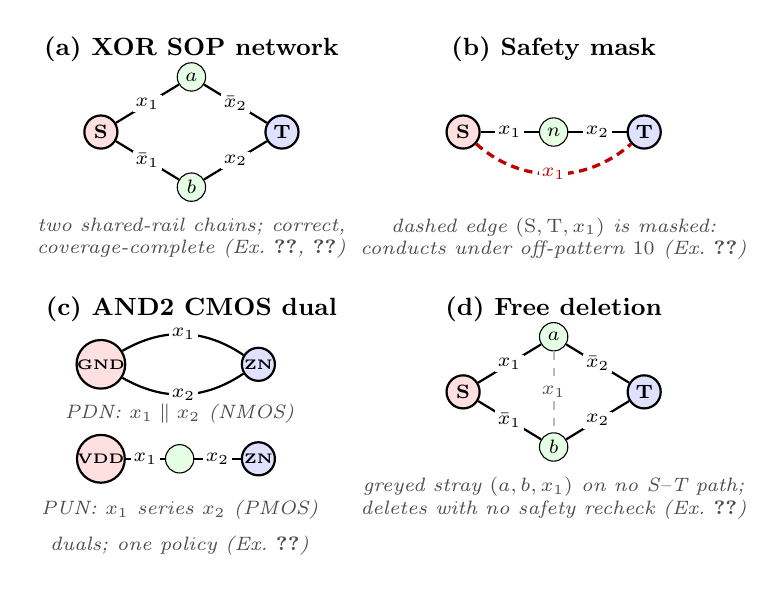
\begin{tikzpicture}[
    font=\scriptsize,
    >=Stealth,
    rail/.style = {circle, draw, thick, minimum size=4.2mm, inner sep=0pt,
                   font=\scriptsize\bfseries},
    src/.style  = {rail, fill=red!12},
    snk/.style  = {rail, fill=blue!12},
    intn/.style = {circle, draw, minimum size=3.6mm, inner sep=0pt, fill=green!10},
    tr/.style   = {draw, thick},
    trlab/.style= {midway, font=\scriptsize, fill=white, inner sep=1pt},
    dead/.style = {draw, thick, gray!55, dashed},
    bad/.style  = {draw, very thick, red!75!black, densely dashed},
    ttl/.style  = {font=\small\bfseries},
    cptn/.style  = {font=\scriptsize\itshape, text=gray!60!black},
]

% ============ (a) XOR SOP network ============
\begin{scope}[shift={(0,0)}]
  \node[ttl] at (1.15,2.05) {(a) XOR SOP network};
  \node[src] (aS) at (0,1.0)   {S};
  \node[snk] (aT) at (2.3,1.0) {T};
  \node[intn] (aa) at (1.15,1.7) {$a$};
  \node[intn] (ab) at (1.15,0.3) {$b$};
  % chain A: S -x1- a -!x2- T
  \draw[tr] (aS) -- node[trlab]{$x_1$} (aa);
  \draw[tr] (aa) -- node[trlab]{$\bar{x}_2$} (aT);
  % chain B: S -!x1- b -x2- T
  \draw[tr] (aS) -- node[trlab]{$\bar{x}_1$} (ab);
  \draw[tr] (ab) -- node[trlab]{$x_2$} (aT);
  \node[cptn, align=center] at (1.15,-0.35)
    {two shared-rail chains; correct,\\ coverage-complete (Ex.~\ref{ex:sop},~\ref{ex:complete})};
\end{scope}

% ============ (b) masked shortcut ============
\begin{scope}[shift={(4.6,0)}]
  \node[ttl] at (1.15,2.05) {(b) Safety mask};
  \node[src] (bS) at (0,1.0)   {S};
  \node[snk] (bT) at (2.3,1.0) {T};
  \node[intn] (bn) at (1.15,1.0) {$n$};
  \draw[tr] (bS) -- node[trlab]{$x_1$} (bn);
  \draw[tr] (bn) -- node[trlab]{$x_2$} (bT);
  % forbidden shortcut S -x1- T (conducts under off-pattern 10)
  \draw[bad] (bS) to[bend right=42] node[trlab, text=red!75!black]{$x_1$} (bT);
  \node[cptn, align=center] at (1.15,-0.35)
    {dashed edge $(\mathrm{S},\mathrm{T},x_1)$ is masked:\\ conducts under off-pattern $10$ (Ex.~\ref{ex:mono})};
\end{scope}

% ============ (c) AND2 dual: PDN vs PUN ============
\begin{scope}[shift={(0,-3.3)}]
  \node[ttl] at (1.15,2.05) {(c) AND2 CMOS dual};
  % PDN: parallel x1 || x2 between GND and ZN
  \node[src] (cG) at (0,1.35) {\tiny GND};
  \node[snk] (cZ1) at (2.0,1.35) {\tiny ZN};
  \draw[tr] (cG) to[bend left=32] node[trlab]{$x_1$} (cZ1);
  \draw[tr] (cG) to[bend right=32] node[trlab]{$x_2$} (cZ1);
  \node[cptn] at (1.0,0.72) {PDN: $x_1 \parallel x_2$ (NMOS)};
  % PUN: series x1 - x2 between VDD and ZN
  \node[src] (cV) at (0,0.15) {\tiny VDD};
  \node[intn] (cm) at (1.0,0.15) {};
  \node[snk] (cZ2) at (2.0,0.15) {\tiny ZN};
  \draw[tr] (cV) -- node[trlab]{$x_1$} (cm);
  \draw[tr] (cm) -- node[trlab]{$x_2$} (cZ2);
  \node[cptn] at (1.0,-0.5) {PUN: $x_1$ series $x_2$ (PMOS)};
  \node[cptn, align=center] at (1.0,-0.95) {duals; one policy (Ex.~\ref{ex:dual})};
\end{scope}

% ============ (d) redundant transistor ============
\begin{scope}[shift={(4.6,-3.3)}]
  \node[ttl] at (1.15,2.05) {(d) Free deletion};
  \node[src] (dS) at (0,1.0)   {S};
  \node[snk] (dT) at (2.3,1.0) {T};
  \node[intn] (da) at (1.15,1.7) {$a$};
  \node[intn] (db) at (1.15,0.3) {$b$};
  \draw[tr] (dS) -- node[trlab]{$x_1$} (da);
  \draw[tr] (da) -- node[trlab]{$\bar{x}_2$} (dT);
  \draw[tr] (dS) -- node[trlab]{$\bar{x}_1$} (db);
  \draw[tr] (db) -- node[trlab]{$x_2$} (dT);
  % stray device a-b, structurally dead -> removed
  \draw[dead] (da) -- node[trlab, text=gray!60!black]{$x_1$} (db);
  \node[cptn, align=center] at (1.15,-0.35)
    {greyed stray $(a,b,x_1)$ on no S--T path;\\ deletes with no safety recheck (Ex.~\ref{ex:reduction})};
\end{scope}

\end{tikzpicture}
}
\caption{Worked $2$-variable circuits for the theoretical results.
(a) The XOR SOP network (Example~\ref{ex:sop}): two shared-rail chains,
correct and coverage-complete, reachable in any insertion order
(Example~\ref{ex:complete}).
(b) A safe series chain for $x_1x_2$; the dashed shortcut $(\mathrm{S},
\mathrm{T},x_1)$ is rejected by the safety mask because it conducts under the
off-pattern $10$ (Example~\ref{ex:mono}).
(c) The AND2 cell: parallel NMOS pull-down, series PMOS pull-up ---
duals synthesized by one policy (Example~\ref{ex:dual}).
(d) A structurally dead transistor (grey), free to delete with no off-pattern
recheck (Example~\ref{ex:reduction}).
Circles S/T are the source/sink rails; small green nodes are internal.}
\label{fig:examples}
\end{figure}

\begin{example}[Decomposing an AND2 cell]
\label{ex:dual}
Let $f = x_1 x_2$, so $\Pon=\{11\}$ and $\Poff=\{00,01,10\}$
(Figure~\ref{fig:examples}(c)).
The CMOS cell splits into two independent switching problems.
The \emph{PDN} realizes $\lnot f$ with on-patterns $\Poff$: it conducts
whenever $x_1{=}0$ or $x_2{=}0$, the \emph{parallel} pair $x_1 \,\|\, x_2$
between $\mathrm{GND}$ and $\mathrm{ZN}$.
The \emph{PUN} realizes $f(\lnot\mathbf{x})$ with on-patterns
$\{\lnot 11\}=\{00\}$: it conducts only when $x_1{=}0$ and $x_2{=}0$, the
\emph{series} pair between $\mathrm{VDD}$ and $\mathrm{ZN}$.
The two networks are duals (series $\leftrightarrow$ parallel), synthesized by
the \emph{same} policy conditioned on their respective pattern sets.
\end{example}

\begin{example}[Monotonicity and incremental safety]
\label{ex:mono}
Take $f = x_1 x_2$, so $\Poff=\{00,01,10\}$.
Suppose the partial network already contains the series pair
(Figure~\ref{fig:examples}(b))
$\SRC \!\xrightarrow{x_1}\! n \!\xrightarrow{x_2}\! \SNK$.
This network is \emph{safe}: under $00$, $01$, $10$ at least one of
$x_1,x_2$ is $0$, so no $\SRC\!\to\!\SNK$ path conducts.
Now add the shortcut $e=(\SRC,\SNK,x_1)$.
By monotonicity (Thm.~2) every previously conducting path still conducts, so
we test only whether $e$ \emph{by itself} creates an off-pattern path
(Cor.~3): under $10\in\Poff$, $x_1=1$, so $e$ alone connects $\SRC$ to $\SNK$
and conducts illegally --- $e$ is masked out.  Adding $e'=(\SRC,\SNK,x_1 x_2)$
would be admissible, since $x_1 x_2 = 0$ on all of $\Poff$.
We reach this verdict by checking only the new edge against $|\Poff|=3$
patterns, never re-examining the existing chain.
\end{example}

\begin{example}[SOP network for a 2-variable function]
\label{ex:sop}
For $f = x_1 \bar{x}_2 + \bar{x}_1 x_2$ (XOR), $\Pon = \{10, 01\}$.
$G_{\mathrm{SOP}}(f)$ places one $2$-transistor chain per on-pattern between
the shared rails (Figure~\ref{fig:examples}(a)): chain~A is
$\SRC\!\xrightarrow{x_1}\!a\!\xrightarrow{\bar{x}_2}\!\SNK$ and chain~B is
$\SRC\!\xrightarrow{\bar{x}_1}\!b\!\xrightarrow{x_2}\!\SNK$.
Under $10$, chain~A conducts and $f=1$; under $01$, chain~B conducts.
Under $00,11$ each chain has one broken transistor, so nothing conducts.
This $4$-transistor network is correct but not minimal --- XOR admits a
$3$-transistor bridge --- and it serves as the fixed \emph{compensate} network
$C_f$ that conditions the state.
\end{example}

\begin{example}[The mask never blocks a valid target]
\label{ex:complete}
Let $G^*$ be the XOR network of Example~\ref{ex:sop} with edges
$\{e_1,e_2\}$ (chain~A), $\{e_3,e_4\}$ (chain~B), built in the interleaved
order $e_1,e_3,e_2,e_4$ that never completes a chain until the end.
At each prefix the partial network is a subgraph of $G^*$; by monotonicity any
off-pattern path in a prefix would also exist in the safe $G^*$, so no prefix
conducts illegally and the mask rejects none of the four placements --- as for
all $4!=24$ orderings.
Thus, although path-order supervision presents one linearization, completeness
guarantees the policy is free to discover $G^*$ in any order.
\end{example}

\begin{example}[A redundant transistor is free to delete]
\label{ex:reduction}
Suppose the policy synthesizes the XOR pull-down of Example~\ref{ex:sop}
(chains A and B) but also emits a stray device $s=(a,b,x_1)$ linking the two
internal nodes (Figure~\ref{fig:examples}(d)).
Deleting $s$ yields $G'\subseteq G$; by Lemma~6 no off-pattern check is
needed, so we re-verify only coverage: chains A and B still carry $10$ and
$01$, hence $G'$ computes the same function.
Because $s$ lies on no \SRC$\to$\SNK path it is structurally dead, and the
reported cost is $T_{\mathrm{eff}}=4$ rather than $5$.
On the $6$-input NSP benchmark this accounting difference is the gap between a
mean of $41.4$ and $19.0$ transistors.
\end{example}

% ============================================================
\section{Proofs}
\label{app:proofs}

\begin{theorem}[Monotonicity of Conducting Paths; Thm.~2]
For any network $G$ and transistor $e \notin E(G)$,
$\mathrm{Paths}(G) \subseteq \mathrm{Paths}(G \cup \{e\})$.
\end{theorem}
\begin{proof}
Adding $e$ can only activate new conducting channels; it cannot deactivate any
already-conducting transistor. Hence every path that conducted in $G$ still
conducts in $G \cup \{e\}$.
\end{proof}

\begin{corollary}[Incremental Safety Checking; Cor.~3]
If $G$ is safe, then $G \cup \{(u,v,\ell)\}$ is safe iff $(u,v,\ell)$ alone
does not create a new $\SRC \to \SNK$ path under any $\pi \in \Poff$.
\end{corollary}
\begin{proof}
Any $\Poff$-path created in $G \cup \{e\}$ must use $e$ (since $G$ was safe),
so checking $e$ alone suffices.
\end{proof}

\begin{theorem}[SOP Network Correctness; Thm.~4]
The series-parallel network with one $N$-transistor series chain per
$\pi \in \Pon$, all sharing $\SRC$/$\SNK$, correctly implements $f$.
\end{theorem}
\begin{proof}
\textit{Coverage}: for $\pi\in\Pon$ all literals in the chain evaluate to 1,
forming a complete path.
\textit{Safety}: for $\pi'\in\Poff$ and chain $\pi\in\Pon$, since $\pi'\neq\pi$
they differ at some bit $j^*$, so the $j^*$-th transistor does not conduct
under $\pi'$, breaking every path.
\end{proof}

\begin{theorem}[Completeness of Safety-Masked Search; Thm.~5]
For any valid $G^*$ implementing $f$, every permutation of $E(G^*)$ is a valid
trajectory under the safety mask.
\end{theorem}
\begin{proof}
Let $e_1,\ldots,e_T$ be any ordering of $E(G^*)$ and $G_t = \{e_1,\ldots,e_t\}$.
\textit{Base}: $G_0=\emptyset$ is safe.
\textit{Step}: if $G_{t-1}$ is safe, then since $G_t \subseteq G^*$ any
$\Poff$-path in $G_t$ would persist in $G^*$ (monotonicity), contradicting
$G^*$'s safety; so $G_t$ is safe and $e_t$ is never rejected.
\end{proof}

\begin{lemma}[Deletion preserves safety; Lem.~6]
Let $G' \subseteq G$ by deleting transistors. If $G$ conducts under no
off-pattern, then neither does $G'$.
\end{lemma}
\begin{proof}
Every path in $G'$ is a path in $G$; a violating path in $G'$ would violate $G$.
\end{proof}

% ============================================================
\section{Hyperparameters}
\label{app:hparam}

\begin{table}[h]
\centering
\caption{Architecture and training hyperparameters.}
\label{tab:hparam}
\begin{tabular}{lc}
\toprule
\textbf{Hyperparameter}          & \textbf{Value} \\
\midrule
MPNN hidden dim $d$              & 128 \\
MPNN layers $L$                  & 3 \\
Head MLP hidden dim              & 256 \\
Post-MPNN self-attention         & yes (4 heads) \\
Node feature dim $d_\mathrm{node}$ & 4 \\
Edge feature dim $d_\mathrm{edge}$ & $N+2$ \ ($5/6/8$ for $N{=}3/4/6$) \\
\midrule
Phase 1 lr (cosine)              & $2\times10^{-3}\!\to\!10^{-4}$ \\
Phase 1 batch size               & 512 \\
Phase 1 epochs                   & 200 \\
Head-1 loss weight               & 2 \\
\midrule
Phase 2 lr                       & $10^{-4}$ \\
Phase 2 trajectories $K$         & 16 \\
PPO clip $\varepsilon$           & 0.2 \\
Entropy coeff $\lambda_H$        & 0.05 \\
Adaptive-anchor $\beta$          & 0.3 \\
Restarts                         & 2 \\
Max updates per target           & 200 \\
Max steps $T_{\max}$             & 20 \\
\midrule
Phase 3 lr                       & $3 \times 10^{-5}$ \\
Phase 3 pairs $K$                & 8 \\
ASTRAN SA quality                & 1 \\
ASTRAN place weights $(w_c, w_m, w_w, w_d, w_g)$ & $(3,4,1,4,2)$ \\
ASTRAN parallel workers          & 4 \\
\bottomrule
\end{tabular}
\end{table}

\end{document}
